\documentclass[11pt]{article}
\usepackage[margin=1in]{geometry}
\usepackage{graphicx}
\usepackage{booktabs}
\usepackage{hyperref}
\usepackage{amsmath}
\usepackage{enumitem}
\usepackage{caption}

\graphicspath{{figures/}{../runs/tiny_real_compare/20260527_153627/}{../runs/tiny_real_compare_long/20260527_155106_1m_long/}{../runs/sparse_attention_study/20260527_161935/}{../runs/mid_arch_ablation/20260527_162441/}}

\title{MiniMax Sparse Attention: A Small MacBook-Scale Research Note}
\author{Vukrosic}
\date{\today}

\begin{document}
\maketitle

\begin{abstract}
This note defines an open-source research program around MiniMax-style sparse attention.
The immediate goal is not to claim a new state-of-the-art model.
The goal is to make a small, inspectable implementation whose routing behavior can be checked, ablated, and compared against dense attention as context length grows.
The current evidence shows that dense and sparse variants remain close on ordinary next-token loss at small scale, while top-$k$ and block size visibly change routing density, throughput, and loss.
That makes the project useful, but unfinished: the central work now is correctness verification, dense-oracle diagnostics, long-context retrieval stress tests, and architecture ablations that explain when sparse routing helps or fails.
\end{abstract}

\section{Goal}
The research question is:
\begin{quote}
Can a block-indexed sparse attention mechanism keep the important context tokens while reducing long-context attention cost, and can we prove that behavior with small reproducible experiments?
\end{quote}

This is different from simply training a small language model and reporting validation loss.
Sparse attention can look fine on short next-token prediction while failing at the job it is supposed to do: preserve useful information from long prefixes.
For that reason, the project has four proof obligations.

\begin{enumerate}[leftmargin=1.5em]
  \item \textbf{Implementation correctness.} The causal mask, block selection, grouped-query mapping, and sparse gather path must match the intended mechanism.
  \item \textbf{Routing fidelity.} The selected blocks should overlap with blocks that dense attention would actually use.
  \item \textbf{Long-context usefulness.} The sparse model should survive longer context windows and retrieval-style probes, not only short training contexts.
  \item \textbf{Ablation clarity.} Each architectural change should answer one question about routing, fallback, reuse, or capacity.
\end{enumerate}

\section{Reference Mechanism}
Figure~\ref{fig:minimax_reference} is the source diagram used as the implementation reference.
The repository does not treat this diagram as a fixed endpoint; it treats it as the first point in a larger sparse-attention design space.
The implementation should therefore be easy to inspect, test, and modify.

\begin{figure}[h]
\centering
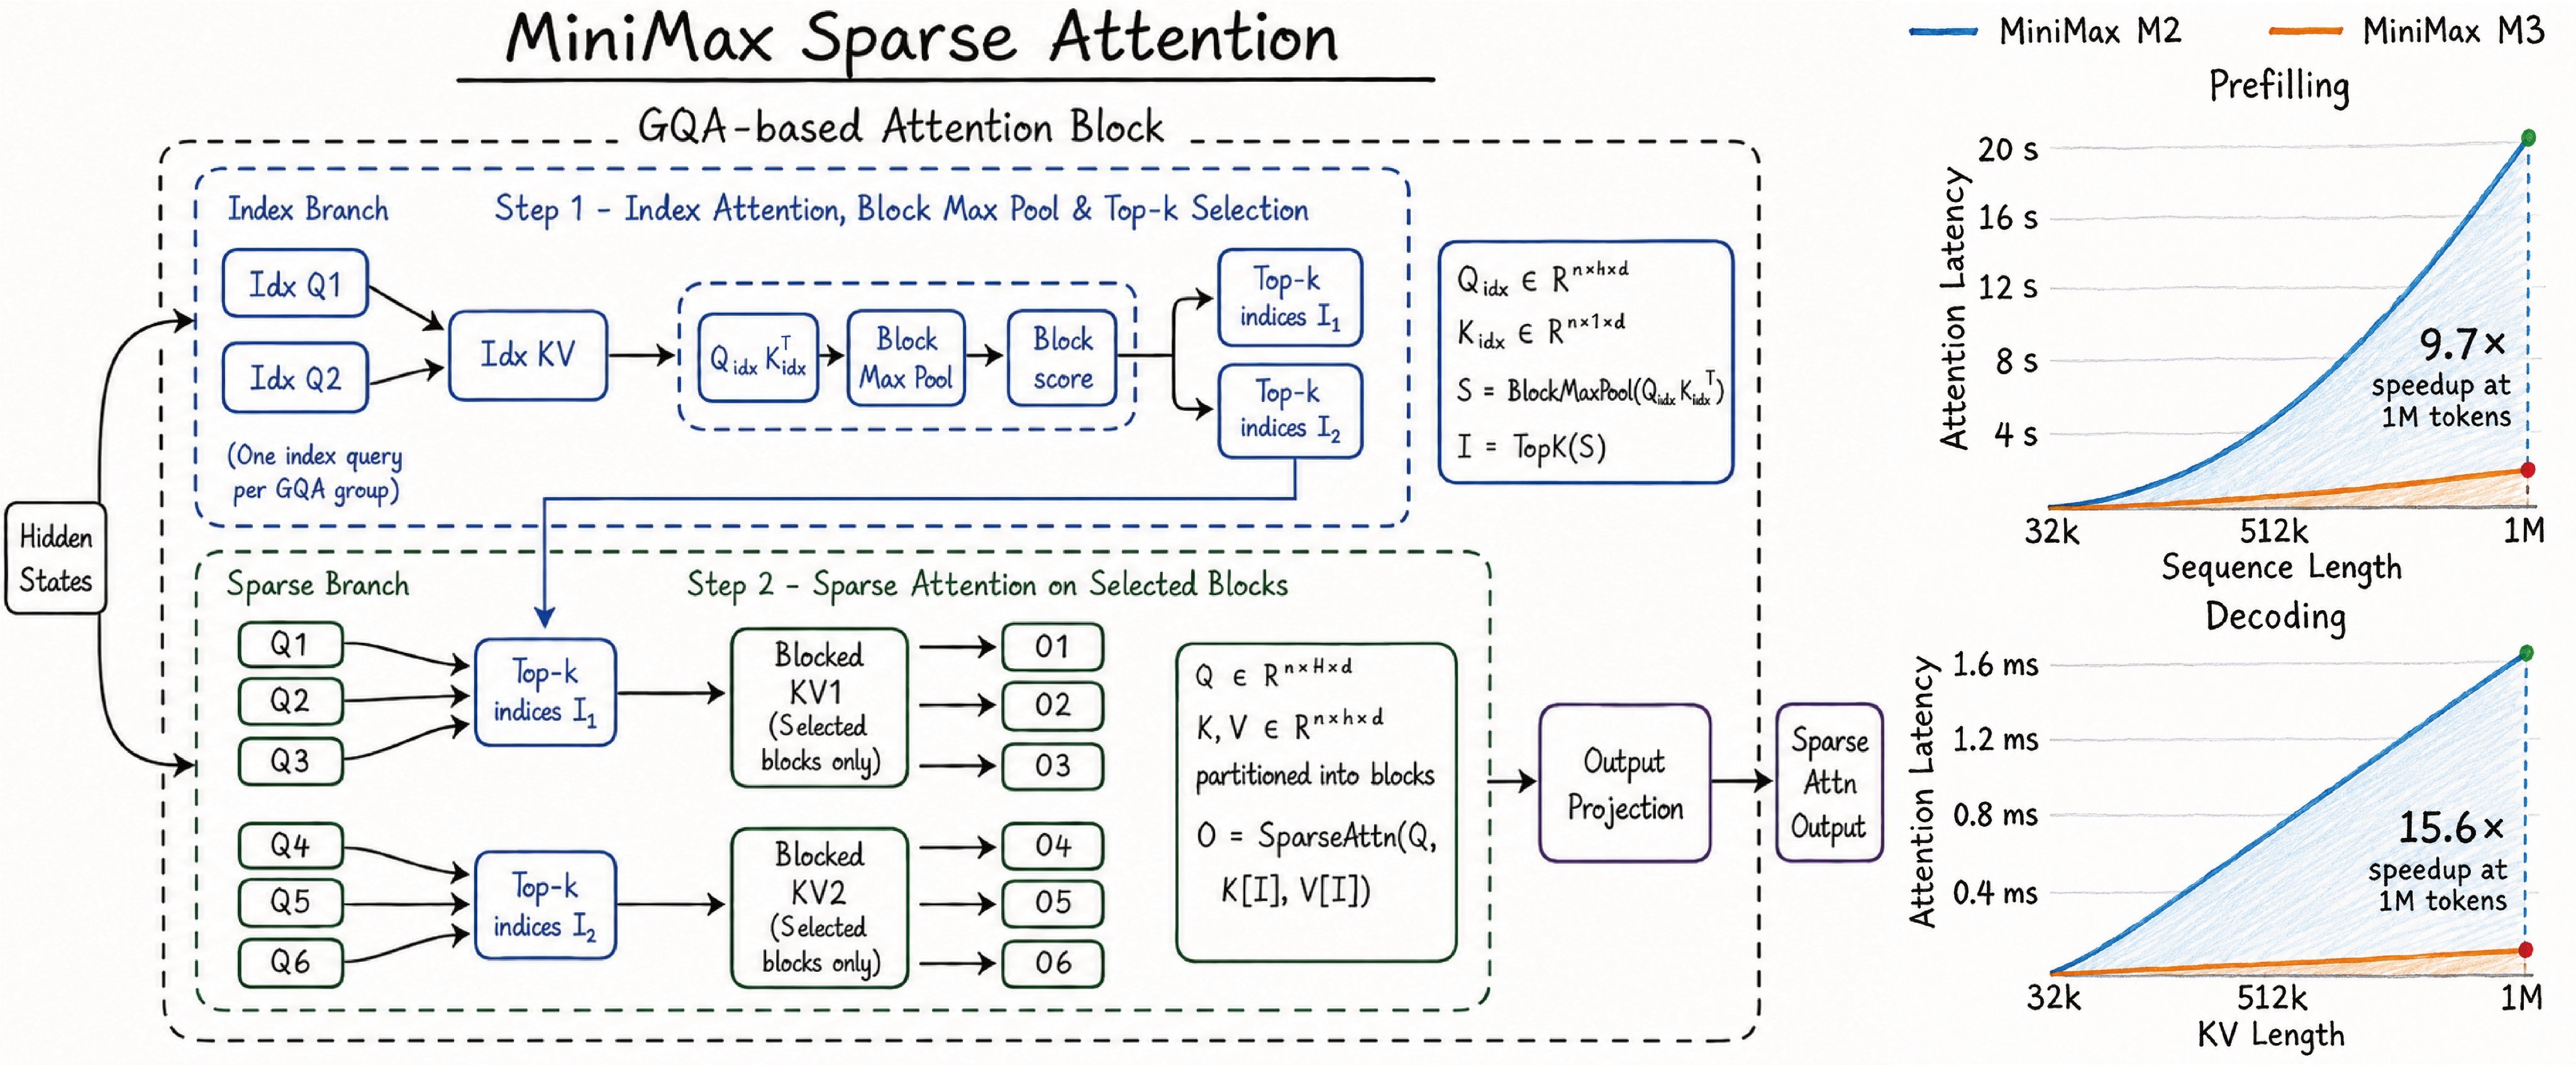
\includegraphics[width=\linewidth]{minimax_sparse_attention_reference.jpg}
\caption{Reference MiniMax-style sparse attention diagram. Source: Skyler Miao X post, \url{https://x.com/SkylerMiao7/status/2059285750458544561}.}
\label{fig:minimax_reference}
\end{figure}

\section{Research Framing}
This paper should be read as an experiment map, not as a final model description.
The router, block size, pooling rule, fallback path, index dimension, GQA grouping, and reuse policy are all candidates for ablation.
If the paper starts by presenting one fixed model, it hides the real scientific question.
The correct framing is that the architecture itself is under test.

The current study keeps the dataset fixed to the real \texttt{speedrun\_40M} subset and uses the same token budget for every run so that differences are easier to attribute to attention design rather than data volume.

\section{Experimental Design}
We organize the work along three axes.

\textbf{Scale.} Three model sizes: the current 5M-class model, a roughly $1.5\times$ larger model, and a roughly $2.25\times$ larger model. This checks whether the sparse mechanism survives capacity changes instead of only working at one size.

\textbf{Context.} Training uses a 256-token sequence length, while evaluation is repeated at 256, 512, and 1024 tokens. This checks whether the routing pattern changes when the prefix gets longer, which is the main reason to study sparse attention at all.

\textbf{Architecture.} The architecture is treated as the object of study, not as a fixed assumption. We compare dense attention with sparse variants that differ in block size, top-$k$, pooling, router projection sharing, local fallback, and reuse.

The smoke runs in this note use AdamW with learning rate $3\times10^{-4}$, weight decay 0.1, gradient clipping at 1.0, batch size 4, and an 80k-token train budget per run.
Evaluation is repeated with four validation batches per context length.
Those settings are deliberately small so contributors can reproduce and modify runs quickly.

\section{Ablation Families}
The paper is built around a small set of ablations that answer different questions.

\textbf{Routing strength.} Vary top-$k$ and block size. This tests whether the router should read a few large regions or more smaller ones.

\textbf{Router scoring.} Vary the pooling operator used by the index branch, for example max, mean, or log-sum-exp. This tests what summary statistic is best for deciding which block survives.

\textbf{Router capacity.} Vary index dimension. This tests whether the router is underpowered, overpowered, or just noisy.

\textbf{Projection sharing.} Compare shared versus separate router/content projections. This tests whether the router should be derived from the attention stream itself or from a separate learned path.

\textbf{Fallback behavior.} Add a local fallback window plus routed blocks. This tests whether sparse attention still needs a dense safety net near the current position.

\textbf{Reuse.} Test cross-layer index reuse. This tests whether routing decisions are stable enough to share across depth instead of recomputing everything each layer.

\textbf{Task stress.} Add long-context retrieval and needle-style probes. This tests whether a sparse router preserves the blocks that matter when the answer is far back in the context.

\section{Open-Source Research Plan}
The project should be contributor-friendly because each useful contribution can be scoped to one proof obligation.
The best issues are not ``improve sparse attention''.
They are concrete checks or ablations with visible artifacts: a failing/passing test, a plot, a JSON result file, or a paper table update.

The first contributor tasks should therefore focus on:
\begin{itemize}[leftmargin=1.25em]
  \item verifying the implementation against the reference mechanism;
  \item adding dense-oracle diagnostics for selected-block recall;
  \item adding a long-context retrieval benchmark where routing quality matters;
  \item testing hybrid local-plus-routed attention;
  \item expanding the router ablation matrix with index dimension and pooling variants;
  \item connecting the paper explanation more directly to the reference image;
  \item improving reproducibility by making every run produce a manifest, command, seed, and plot.
\end{itemize}

This gives contributors a reason to stay: each task is small enough to finish, but each one changes the research conclusion.
The repository should reward contributions that make claims more checkable, not just contributions that add code.

\section{What Is Under Test}
Only after the design axes are clear do we state the attention family itself.

The implementation is a compact PyTorch sparse-attention block inspired by the diagrammed MiniMax structure:
an index branch scores KV blocks, applies causal pooling, and selects the top-$k$ blocks;
the sparse branch then attends only over the selected blocks.
The code is intentionally unfused so the paper can focus on architecture and experimental behavior before any kernel work.

\subsection{Components}
The attention family has four separable pieces.

\textbf{Base transformer shape.} The decoder scaffold: embedding width, number of layers, head count, KV head count, and feedforward width. This is the capacity axis.

\textbf{GQA backbone.} Grouped-query attention reduces KV cost while preserving multi-head query structure. This is the backbone the sparse mechanism sits on.

\textbf{Index branch.} The lightweight router scores blocks and selects the top-$k$ candidates for each query group. This is the part that decides which memory survives.

\textbf{Sparse branch.} The content branch attends only over the selected blocks. Different pooling rules, local fallback behavior, and reuse strategies can all be plugged into this branch family.

\section{Related Work}
Sparse attention has several nearby ancestors. Sparse Transformer introduced hand-designed sparse factorizations and showed that structured sparsity can extend autoregressive modeling to much longer contexts than dense attention \cite{child2019sparse}. Longformer and BigBird combined local windows with global or random links for long-document modeling, and BigBird added theoretical coverage guarantees \cite{longformer2020,bigbird2020}. Reformer and Routing Transformer took a more content-based route, using locality-sensitive hashing or online clustering to group similar tokens together \cite{reformer2020,routing2020}.

Grouped-query attention is orthogonal but important here: it reduces key/value cost without making attention sparse, which is why our sparse block sits on top of a GQA backbone rather than replacing it \cite{gqa2023}. Recent production-scale work moves closer to our setup. MoBA routes queries to a few KV blocks and reports that block size and router design matter; NSA combines coarse token compression with finer token selection; and IndexCache shows that sparse index decisions can sometimes be reused across layers with little quality loss \cite{moba2025,nsa2025,indexcache2026}.

\section{Results}
Table~\ref{tab:main} summarizes the two key runs so far.

\begin{table}[h]
\centering
\caption{Real-data smoke results.}
\label{tab:main}
\begin{tabular}{lrrrrr}
\toprule
Model & Tokens & Seconds & Val loss & Val ppl & Tok/s \\
\midrule
500k dense & 501,760 & 88.49 & 7.4787 & 1769.88 & 5,650 \\
500k sparse & 501,760 & 69.11 & 7.4860 & 1782.89 & 7,234 \\
1M dense & 1,001,472 & 92.00 & 6.8665 & 959.54 & 10,886 \\
1M sparse & 1,001,472 & 127.24 & 6.8866 & 979.05 & 7,871 \\
\bottomrule
\end{tabular}
\end{table}

Figure~\ref{fig:short} shows the 500k-token comparison and Figure~\ref{fig:long} shows the longer 1M-token run with tagged panels.

\begin{figure}[p]
\centering
\includegraphics[width=\linewidth]{comparison.png}
\caption{500k-token dense vs sparse smoke run. The curves look close because the loss gap is small relative to the full loss range.}
\label{fig:short}
\end{figure}

\begin{figure}[p]
\centering
\includegraphics[width=\linewidth]{comparison_1m_long.png}
\caption{1M-token dense vs sparse run. The delta panel shows the sparse model stays close but does not beat dense on validation loss in this run.}
\label{fig:long}
\end{figure}

\section{Additional Sweep Results}
We then ran the study sweep across three model scales and three evaluation context lengths. The main takeaways are simple: larger models help more than router tweaks, and the 1024-token evaluation does not collapse relative to 256 in this small-budget regime.

Figure~\ref{fig:study} summarizes the scale/context sweep. Across the current, mid, and large settings, dense remains slightly ahead of sparse on the same token budget, but the gap stays small and the longer-context evaluation remains stable.

\begin{figure}[p]
\centering
\includegraphics[width=\linewidth]{study_summary.png}
\caption{Scale and context sweep. Each panel shows validation loss versus context length for one model scale.}
\label{fig:study}
\end{figure}

The more interesting architectural signal came from the mid-scale router sweep. Pooling style and shared-router projection barely changed the selected blocks on a held-out real batch, so the more diagnostic knobs were block size and top-$k$.

\begin{table}[p]
\centering
\caption{Mid-scale sparse-attention architecture ablation on the real 40M slice. Density and selected-block counts are probe measurements on a held-out real batch.}
\label{tab:arch}
\begin{tabular}{lrrrr}
\toprule
Variant & Val loss & Tok/s & Probe density & Mean selected blocks \\
\midrule
top-$k=1$ & 8.2111 & 4896 & 0.2288 & 1.00 \\
top-$k=2$ & 8.2051 & 4764 & 0.3742 & 1.94 \\
top-$k=4$ & 8.2023 & 4202 & 0.5860 & 3.62 \\
block size 8 & 8.2052 & 5226 & 0.2290 & 1.97 \\
block size 32 & 8.2076 & 4440 & 0.5771 & 1.88 \\
\bottomrule
\end{tabular}
\end{table}

Figure~\ref{fig:arch} shows the matching architecture-ablation curves.

\begin{figure}[p]
\centering
\includegraphics[width=\linewidth]{arch_summary.png}
\caption{Mid-scale architecture ablation. Top-$k$ and block size change the routing density and the final loss more than pooling or shared-router projection did in this run.}
\label{fig:arch}
\end{figure}

\section{Analysis}
The main result is not that sparse attention wins. It does not, at least not yet.
Instead, the current evidence says:
\begin{itemize}[leftmargin=1.25em]
  \item The sparse router is real and changes the computation path.
  \item On ordinary next-token loss, dense and sparse remain very close at this scale.
  \item The sparse model is not obviously better on quality, and throughput depends on the backend.
  \item The delta is small enough that plotting only a single loss curve is misleading.
  \item Pooling style and shared-router projection were too weak to separate cleanly at this budget; top-$k$ and block size were the better architectural knobs.
\end{itemize}

The attention diagnostics also show the sparse path differs from dense in logits and routing density, so the near-overlap in training curves is not an implementation collapse.
That makes this a good setup for ablations, not a dead end.

\section{Open Questions and Ablations}
The current runs say dense and sparse are close on short next-token loss, so the main question is no longer whether the router exists. The question is where the router helps, where it misses, and how much of the gain is routing quality versus backend efficiency.

The most informative follow-up experiments on this MacBook are:
\begin{itemize}[leftmargin=1.25em]
  \item vary top-$k$ at fixed block size
  \item vary block size at fixed top-$k$
  \item vary index dimension
  \item vary the pooling operator used by the index branch, for example max, mean, or log-sum-exp
  \item vary the number of KV heads and the query-to-KV grouping ratio
  \item compare shared versus separate projections for the router and the content branch
  \item add a local fallback window plus routed blocks to test whether near-context continuity matters
  \item test cross-layer index reuse, inspired by IndexCache, to see whether router outputs are stable enough to cache
  \item compare hard top-$k$ selection with a softer or temperature-controlled router
  \item compare dense vs sparse across three seeds
  \item add a long-context retrieval task where the queried answer sits many blocks earlier
\end{itemize}

For each ablation, the useful measurements are validation loss, perplexity, throughput, selected-block density, router entropy, selected-block recall against a dense oracle probe, and long-context retrieval accuracy.

\section{Limitations}
This is still a small-scale, unfused PyTorch study.
It does not yet test the very long context regime from the MiniMax diagram, and it does not isolate whether any gain comes from routing quality or from backend-specific effects.
That is fine for a first pass, but it means we should treat the current result as a research scaffold rather than a conclusion.

\section{Conclusion}
The project is in the useful middle state: the baseline is real, the sparse architecture is real, the plots are real, and the differences are measurable but modest.
The next paper update should be about ablation curves, routing diagnostics, and a retrieval benchmark, not another generic next-token smoke run.

\begin{thebibliography}{99}
\bibitem{vaswani2017}
Ashish Vaswani et al.
\newblock Attention Is All You Need.
\newblock \url{https://arxiv.org/abs/1706.03762}

\bibitem{child2019sparse}
Rewon Child, Scott Gray, Alec Radford, and Ilya Sutskever.
\newblock Generating Long Sequences with Sparse Transformers.
\newblock \url{https://arxiv.org/abs/1904.10509}

\bibitem{longformer2020}
Iz Beltagy, Matthew E. Peters, and Arman Cohan.
\newblock Longformer: The Long-Document Transformer.
\newblock \url{https://arxiv.org/abs/2004.05150}

\bibitem{bigbird2020}
Manzil Zaheer et al.
\newblock Big Bird: Transformers for Longer Sequences.
\newblock \url{https://arxiv.org/abs/2007.14062}

\bibitem{reformer2020}
Nikita Kitaev, \L ukasz Kaiser, and Anselm Levskaya.
\newblock Reformer: The Efficient Transformer.
\newblock \url{https://arxiv.org/abs/2001.04451}

\bibitem{routing2020}
Aurko Roy et al.
\newblock Efficient Content-Based Sparse Attention with Routing Transformers.
\newblock \url{https://arxiv.org/abs/2003.05997}

\bibitem{gqa2023}
Joshua Ainslie et al.
\newblock GQA: Training Generalized Multi-Query Transformer Models from Multi-Head Checkpoints.
\newblock \url{https://arxiv.org/abs/2305.13245}

\bibitem{moba2025}
Enzhe Lu et al.
\newblock MoBA: Mixture of Block Attention for Long-Context LLMs.
\newblock \url{https://arxiv.org/abs/2502.13189}

\bibitem{nsa2025}
Jingyang Yuan et al.
\newblock Native Sparse Attention: Hardware-Aligned and Natively Trainable Sparse Attention.
\newblock \url{https://arxiv.org/abs/2502.11089}

\bibitem{indexcache2026}
Yushi Bai et al.
\newblock IndexCache: Accelerating Sparse Attention via Cross-Layer Index Reuse.
\newblock \url{https://arxiv.org/abs/2603.12201}
\end{thebibliography}

\end{document}
